\documentclass[12pt]{article}
\usepackage{fancyhdr}
\usepackage{graphicx}
\usepackage{natbib}

%NB: fancyhdr pkg also has commands for messing with margin,
% plus nice diagram of what the below commands mean
\hoffset=-0.75in
\voffset=-0.75in
\textwidth=7in
\textheight=9.5in
\topmargin=0in

%\pagestyle{fancy}
%\rhead{Mapping the nearest  galaxy filament}
%\lhead{\thepage}
%\renewcommand{\headrulewidth}{0pt}


\begin{document}

\pagestyle{empty}

% this doesn't actually go here but it's a good way to keep it together.
\section*{Abstract}
The NGC~3109 association is a nearly-linear group of dwarf galaxies located at the edge of the Local Group. 
The origin of this group is as yet unclear: is it an infalling dark matter filament, a set of `backsplash' galaxies
which have passed through the Milky Way in the past, or a group of tidal dwarfs formed in a past Milky Way/M31
encounter? Distinguishing among these possibilities requires a complete accounting of the galaxies in
the group, their star formation histories, and their kinematics. Several members of the NGC~3109 association 
have only  recently been discovered, and we propose a deep MegaCam survey to search for additional galaxies.
*Stirring final sentence here*.


\clearpage


\section*{Science Justification}
The large scale structure of our local universe is dominated by voids and filamentary structures of groups and clusters of galaxies 
(e.g., Courtois et al.\ 2013).  Half of the Local Volume galaxies reside in loose groups and associations, such as the Sculptor filament 
and the Canes Venatici Cloud (Karachenstev 2005). The nearest such structure is the NGC~3109 association (see Figure 1), an
 association of 5 dwarf galaxies in Leo, Sextans, and Antlia (van den Bergh 1999; Tully et al.\ 2006). This galaxy association, 
 with a linear extent of 1.2~Mpc across the sky (Bellazzini et al.\ 2013), lies just at the edge of the Local Group at a distance of 
 1.3--1.7 Mpc. The origin of the NGC~3109 association is discussed in detail by Pawlowski \& McGaugh (2014), who identify 
 several possibilities: an infalling dark matter filament, a  pre-existing group tidally stretched by an encounter with the MW, or galaxies
 formed as tidal dwarfs from a past Milky Way/M31 encounter. Constraining the number and properties  of additional group
 members can help to discriminate between these possibilities as well as confirm or refute the suggestion by Pawlowski \& McGaugh (2014)
 that {\em all} of the non-satellite galaxies to the north of the Milky Way are confined to a single plane.

The time is right for a search for additional members of the NGC~3109 association. While the region is covered by existing  and planned
survey data, none are deep enough to detect the faint galaxies and  structures at this distance. The most
well-known recent examples of nearby dwarf galaxy discovery are from the SDSS (e.g., Koposov et al.\ 2008).
However, despite lying within the SDSS footprint, the newest member of the NGC~3109 association, Leo P, 
was recently discovered as part of a blind H~I survey (Giovanelli et al.\ 2013): it is simply too faint to
be well-detected at the SDSS  depth ($g=22.2$, $i=21.3$)
%This galaxy has an H~I mass of $10^6$ solar masses and a stellar mass about $3\times10^5$~M$_{\odot}$, and is extremely metal-poor:
Using LBT imaging of Leo~P, McQuinn et al.\ (2013) measured the tip of its red giant branch to be at $i=22.1$.
Further south, tidal substructure near the Antlia dwarf suggestive of an interaction with NGC~3109 was recently discovered by Penny et al.\ (2012),
at very low surface brightness levels.
This suggests to us that additional  faint members of the group as well as tidal debris from interactions between group members 
may await discovery.

The outcome of a search for additional members of the NGC~3109 association has important implications for
understanding galaxy evolution. A lack of additional tidal debris could cast doubt on the `tidal dwarf' 
explanation for the group's existence, while a lack of additional bound-galaxy members of the group 
would strongly constrain the mass of a possible dark-matter filament or progenitor halo.
On the other hand, finding additional members of the group would allow a better characterization of its
spatial and dynamical extent; with only five currently-identified members, such studies 
suffer from small-number statistics. If additional group members lie close to the same plane
as the existing members, this would tend to confirm the result of Pawlowski \& McGaugh (2014). 
Identification of new members as potential `backsplash galaxies' (Teyssier et al.\ 2012) might lend credence to 
 Pawlowski \& McGaugh's
claim that there is an `overabundant backsplash galaxy' problem with $\Lambda$CDM.
Additional group members 
would also allow better constraints on the group's  luminosity function and subsequent comparison to CDM 
simulations of galaxy formation in  low-density environments.

%A discussion of how the observations will constrain the underlying theory is also missing: are additional (presumably HI-deficient) satellites or stellar streams expected theoretically, and what are the implications if they are or are not found? 


% Filamentary structures are considered to be in an earlier stage of their evolution, thus a complete characterization of the interacting environment of the NGC~3109 structure will provide us with insights to lend interpretation to more distant structures, such as the Sculptor filament (e.g. Jerjen et al.\ 1998).

The southern part of the NGC~3109 filament, from NGC~3109 to Sextans B, is expected to be observed with LSST.
The northern portion of  the NGC~3109 filament, from Sextans B to Leo P, requires deeper imaging than
the available  SDSS  depth ($g=22.2$, $i=21.3$) in order to detect dwarf galaxies at distances beyond 1 Mpc.
CFHT/MegaCam's ability to go both wide and deep is essential for such observations: the nearby nature of the 
filament means that it covers a large area of sky, yet the expected faint dwarf galaxies are resolved into individual stars.


Completing the substructure census and probing the faintest end of the luminosity function in the nearest filamentary 
structure are the goals of this proposal. Detected low-surface brightness structures will be characterized in terms of 
structural properties and their association to the sub-group will be pursued via tip-of-the-red-giant-branch 
(TRGB; Lee et al.\ 1993) measurements and, if possible, kinematical measurement.


%\clearpage
\thispagestyle{empty}


\begin{figure}
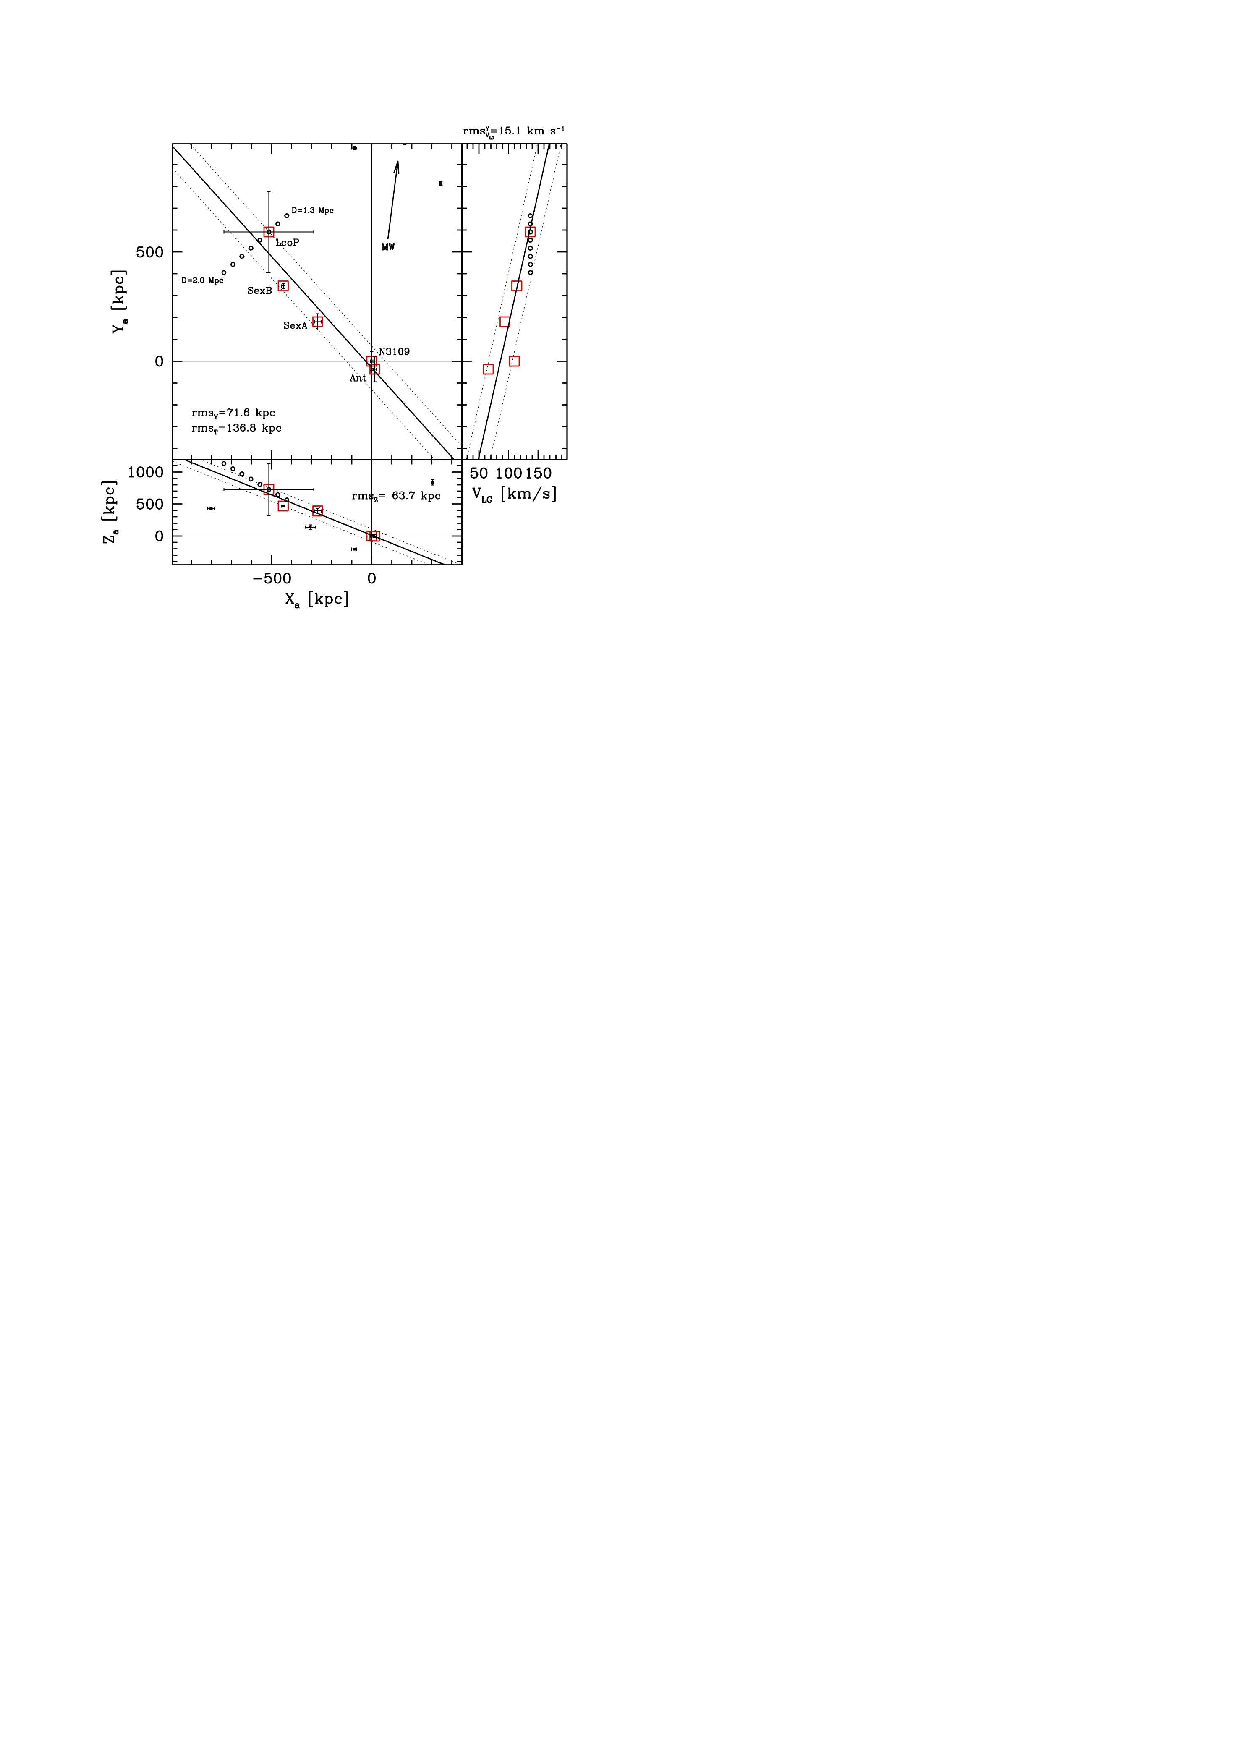
\includegraphics[scale=0.5]{bellaz_fig1}
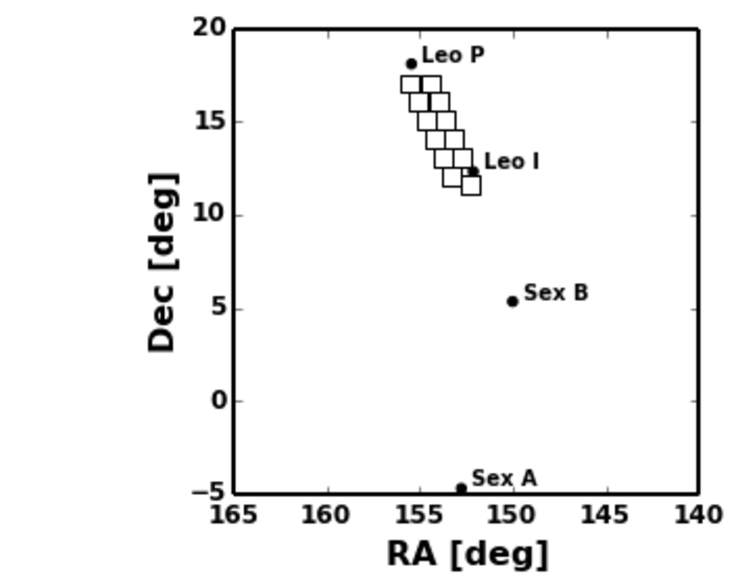
\includegraphics[scale=0.5]{fields_leoi_new}
%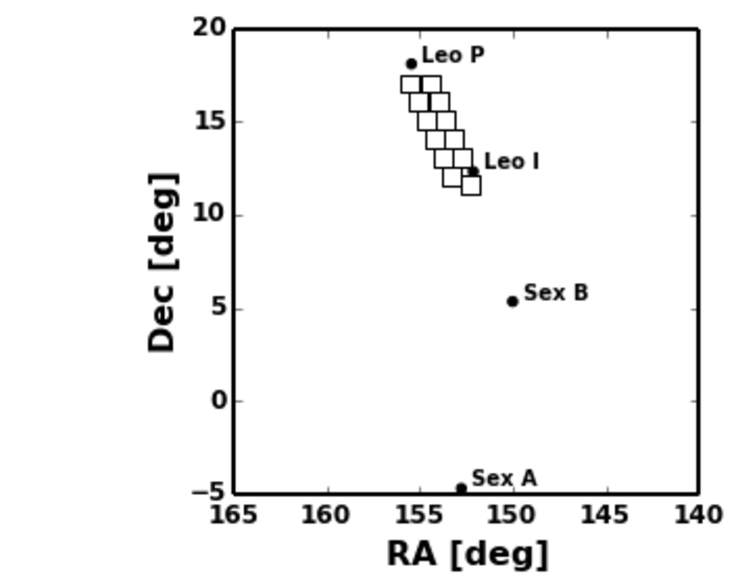
\includegraphics[scale=0.5]{fields_leoi_new}
\caption{(Left) The NGC 3109 association shown in Cartesian coordinates centred on NGC 3109,  from Bellazzini et al.\ (2013).
(Right) Sky projection of the proposed observations. The boxes are 1-degree MegaCam fields; the black circles at the galaxy
locations have 15-arcminute radii. 
}
\end{figure}



% get these ordered correctly at end
\section*{References}

\begin{table}[h]
\begin{tabular}{ll}
Bellazzini, M. et al.\  2013, A\&A 559, L11 & Pawlowski, M.S. \&  McGaugh, S.S. 2014, MNRAS, 440, 908\\
Bellazzini, M. et al.\  2014, A\&A 566, 44 & Koposov, S. et al.\ 2008, ApJ, 686, 279\\
Chiboucas, K. et al.\  2009, AJ, 137, 3009 & Lee, M.G. et al.\ 1993, ApJ, 417, 993\\
Courtois, H.R. et al.\ 2013, AJ, 146, 69 &  McQuinn, K.B.W. et al. 2013, AJ, 146, 145\\
Giovanelli, R. et al.\ 2013, AJ, 146, 15 & Penny, S.J. et al. 2012, ApJ, 758, L32\\
Jerjen, H. et al.\ 1998, AJ, 116, 2873  &  Tully, R.B. et al.\ 2006, AJ, 132, 729\\
Karachentsev, I. 2005, AJ, 129, 178 &van den Bergh, S. 1999, ApJ, 517, L97\\
Keller, S.C. et al.\ 2007, PASA, 24, 1 & Sohn, S.T. et al.\ 2007, ApJ, 663, 960\\
{Pe{\~n}arrubia}, J. et al.\ 2009, ApJ, 298, 222 & Teyssier, M. et al.\ 2012, MNRAS, 426, 1808
\end{tabular}
\end{table}


% Begyu et al.\ 2013, AJ 145, 120\\ % "AN INTERACTING GALAXY SYSTEM ALONG A FILAMENT IN A VOID "
%Bellazzini, M. et al.  2013, A\&A 559, L11\\
%Chiboucas, K. et al.\  2009, AJ, 137, 3009\\
%Courtois, H.R. et al.\ 2013, AJ, 146, 69\\
%Giovanelli, R. et al.\ 2013, AJ, 146, 15\\
%Jerjen, H. et al.\ 1998, AJ, 116, 2873\\
%Karachentsev, I. 2005, AJ, 129, 178 \\
%Keller, S.C. et al.\ 2007, PASA, 24, 1\\
%Koposov, S. et al.\ 2008, ApJ, 686, 279\\
%Lee, M.G et al.\ 1993, ApJ, 417, 993\\ 
%McQuinn, K.B.W. et al. 2013, AJ, 146, 145\\
%Penny, S.J. et al. 2012, ApJ, 758, L32\\
%Tully, R.B. et al.\ 2006, AJ, 132, 729\\
%van den Bergh, S. 1999, ApJ, 517, L97\\



\clearpage
% tech justification goes here.

%\thispagestyle{empty}

\section*{Technical Justification}
As defined by Bellazzini et al.\ (2013), the NGC~3109 filament is  distributed along a line extending from Leo P in the 
north ($\delta = +18^{\circ}$, $b = +54^{\circ}$) to
Antlia in the south ($\delta = -27^{\circ}$, $b = +22^{\circ}$); Sextans B is about 3$^{\circ}$ to the west of this line.
While galaxies belonging to the NGC~3109 association might not lie along the filament defined by
the 5 known members, the structure provides the most obvious `lamp post' under which to search for new
members. The southern part of the filament will be observed with LSST (coverage to $\delta < +10^{\circ}$ to the necessary depth),
but the northern portion is out of LSST's reach. The SDSS coverage of the northern portion of the filament
is of insufficient depth for our purposes.
We have defined a series of Megacam pointings covering a $2^{\circ}\times6^{\circ}$ region south
of Leo~P in the direction towards Sextans~A~and~B; see Figure 2. This area subtends $44\times136$~kpc
at the distance of the NGC~3109 association; for comparison, the tidal truncation radius of Sextans~A is
about 3~kpc (Bellazzini et al.\ 2014). As the Figure shows,  our defined fields are also
quite close to the more nearby (240~kpc) dwarf galaxy Leo~I and can be used to probe the outer
regions of this galaxy. The position of the field nearest Leo~I has been adjusted slightly to avoid the
bright star Regulus.


Megacam imaging in two filters is important for separating the giant branches of additional NGC~3109
members from both foreground Galactic stars and background unresolved galaxies.  Bellazzini et al.\ (2013, 2014)
successfully demonstrated the ability to effectively remove contamination using colour information
in an LBT study of Sextans A and B in $g$ and $r$. Of the MegaCam filters, the $r$ band is best-matched to the SED 
peak of red giants in an old stellar population.
The imaging depth is set by the requirement to detect enough stars for a significant measurement of overdensity. 
With data reaching 3 magnitudes below the TRGB, McQuinn et al.\ (2013) found Leo P to have a {\em central} surface brightness 
of $\mu_V=24.5$~mag~arcsec$^2$ and only a few hundred RGB stars. We aim to reach 
a depth of two magnitudes below the TRGB ($M_r = -3.1$, or  $r=23$ at 1.7~Mpc), meaning $r=25$;
this is shallower than the Bellazzini et al.\  data, but their fainter objects were dominated by background galaxies. 
The $g-r$ colour found by Bellazzini et al.\ at $r=25$ was $g-r\approx 1.0$ so the required $g$-band depth is $g=26$.

We will search for new, faint members of the NGC~3109 association using the standard methods in the field:
searching for spatial overdensities of resolved stars within magnitude and colour ranges expected for the stellar populations.
The resolved stellar population studies of known NGC~3109 group members provide excellent templates for
this work. Foreground and background (stellar and galaxy) populations are also well-characterized in these
studies and others, so filtering out only the populations of interest is feasible.

To estimate exposure times, we assume less-than-perfect conditions (dark time, 1 arcsec seeing, airmass 1.2, 90\% transparency)
since our proposed observations  overlap in RA with Large Programs MATLAS and LUAU and we have not
tightly constrained the observing
conditions. Assuming overheads for 4 dithered exposures per filter, reaching 
$r=25$ and $g=26$ at $S/N=5$ requires 1.5 hours per field (0.5 in $r$ and 1.0 in $g$.)
(We note that in their successful Megacam detection of more than a 
dozen dwarf galaxies in the M81 group, Chiboucas et al.\ (2009) had somewhat
better conditions than assumed here and reached $r=25$ in approximately 1200~s exposures.)
We therefore request a total of 18 hours of exposure time.





\end{document}
